Έστω τώρα ότι η πραγματική και η εκτιμώμενη στάση είναι ίσες ως προς τον
προσανατολισμό $\hat{\theta} = \theta$, αλλά άνισες ως προς τη θέση
$\hat{\bm{l}} \neq \bm{l}$. Εάν ο χάρτης αναπαριστά το περιβάλλον τέλεια και ο
φυσικός αισθητήρας αναφέρει μετρήσεις χωρίς διαταραχές, τότε η εκτίμηση της
θέσης του αισθητήρα μπορεί να οδηγηθεί αυθαίρετα κοντά στην πραγματική θέση. Σε
πραγματικές συνθήκες, όταν οι ακτίνες των πραγματικών σαρώσεων ή/και των
εικονικών σαρώσεων αλλοιώνονται από προσθετικό θόρυβο πεπερασμένου μέγιστου
μέτρου, η εκτίμηση θέσης μπορεί να φραχθεί σε μια γειτονιά της πραγματικής
θέσης του αισθητήρα. Τα θεωρήματα \ref{prop:theorem_without_disturbance} και
\ref{prop:theorem_with_disturbance} τυποποιούν αυτές τις δηλώσεις
\cite{Filotheou2022d}.


\begin{bw_box}
\begin{theorem}
  \label{prop:theorem_without_disturbance}

  Έστω ότι ισχύουν οι υποθέσεις του προβλήματος \ref{}??, και ότι
  $\hat{\theta} = \theta$. Έστω επίσης ότι η εικονική σάρωση $\mathcal{S}_V$ που
  συλλαμβάνεται από τη στάση $\hat{\bm{p}}$ εντός του χάρτη $\bm{M}$
  συμβολίζεται με $\mathcal{S}_V|_{\bm{\hat{p}}}$. Έστω ακόμα ότι οι
  δισδιάστατες σαρώσεις $\mathcal{S}_R$ και $\mathcal{S}_V$ είναι απαλλαγμένες
  από διαταραχές, δηλαδή ότι οι αποστάσεις που καταγράφουν οι ακτίνες της
  πραγματικής σάρωσης προς τα γύρω του εμπόδια αντιστοιχούν στις πραγματικές
  αποστάσεις του αισθητήρα από τα εν λόγω εμπόδια, και ότι ο χάρτης του
  περιβάλλοντος το αναπαριστά τέλεια. Αντιμετωπίζοντας την
  εκτίμηση της θέσης του αισθητήρα ως μεταβλητή κατάστασης
  $\hat{\bm{l}}[k] = [\hat{x}[k], \hat{y}[k]]^\top$ και ενημερώνοντάς την
  σύμφωνα με την εξίσωση διαφορών
  \begin{align}
    \hat{\bm{l}}[k+1] = \hat{\bm{l}}[k] + \bm{u}[k]
    \label{eq:difference_equation_without_disturbance}
  \end{align}
  όπου $\hat{\bm{l}}[0] = \hat{\bm{l}} = [\hat{x}, \hat{y}]^{\top}$,
  (δηλαδή η παρεχόμενη αρχική εκτίμηση της θέσης), $\bm{u}$ είναι ένα διάνυσμα
  διαστάσεων $2 \times 1$ που στο εξής θα αναφέρεται ως
  \textit{διάνυσμα ελέγχου}:
  \begin{align}
    \bm{u}[k] = \dfrac{1}{N_s}
    \begin{bmatrix}
      \cos\hat{\theta} & \sin\hat{\theta} \\\
      \sin\hat{\theta} & - \cos\hat{\theta}
    \end{bmatrix}
    \begin{bmatrix}
      X_{1,r}\big(\mathcal{S}_R, \mathcal{S}_V|_{\bm{\hat{p}}[k]}\big) \vspace{0.2cm} \\
      X_{1,i}\big(\mathcal{S}_R, \mathcal{S}_V|_{\bm{\hat{p}}[k]}\big)
    \end{bmatrix}
    \label{eq:control_vector_without_disturbance}
  \end{align}
  όπου $X_{1,r}(\cdot)$ και $X_{1,i}(\cdot)$ είναι, αντίστοιχα, το πραγματικό
  και φανταστικό μέρος της μιγαδικής ποσότητας $X_1$:
  \begin{align}
    X_1\big(\mathcal{S}_R, \mathcal{S}_V|_{\bm{\hat{p}}[k]}\big) &= X_{1,r}\big(\mathcal{S}_R, \mathcal{S}_V|_{\bm{\hat{p}}[k]}\big)
      + i \cdot X_{1,i}\big(\mathcal{S}_R, \mathcal{S}_V|_{\bm{\hat{p}}[k]}\big) \nonumber \\
      &= \sum\limits_{n=0}^{N_s-1}(\mathcal{S}_R[n] - \mathcal{S}_V[n]|_{\bm{\hat{p}}[k]}) \cdot e^{-i \frac{2 \pi n}{N_s}} \label{eq:X1}
  \end{align}
  όπου $\mathcal{S}_R[n]$ και $\mathcal{S}_V[n]|_{\bm{\hat{p}}[k]}$ είναι,
  αντίστοιχα, οι αναφερόμενες αποστάσεις της $n$-οστής ακτίνας της πραγματικής
  $\mathcal{S}_R$ και εικονικής σάρωσης $\mathcal{S}_V|_{\bm{\hat{p}}[k]}$, και
  $\hat{\bm{p}}[k] = (\hat{\bm{l}}[k], \hat{\theta})$---τότε η εκτίμηση θέσης
  $\hat{\bm{l}}[k]$ \textit{συγκλίνει ομοιόμορφα ασυμπτωτικά στην πραγματική
  θέση} $\bm{l}$ \textit{καθώς} $k \rightarrow \infty$.
\end{theorem}
\end{bw_box}

Στην πράξη το σύστημα ελέγχου
(\ref{eq:difference_equation_without_disturbance},
\ref{eq:control_vector_without_disturbance}) αφήνεται να επαναληφθεί είτε
έως ότου το μέτρο του διανύσματος ελέγχου $\bm{u}[k]$ φτάσει σε ένα επαρκώς
μικρό μέγεθος $\|\bm{u}[k]\|_2 < \varepsilon_u$, όπου $\varepsilon_u$ είναι
επαρκώς μικρό---π.χ. $\varepsilon_u < 10^{-3}$---ή για $I_T > 0$ επαναλήψεις
(ένα αρκετά μεγάλο, εξωτερικά παρεχόμενο όριο μέγιστων επαναλήψεων---π.χ. $I_Τ
\geq 20$). Επομένως, συμβολίζοντας με $k_{stop} \in (0, I_T]$ τον δείκτη
της τελευταίας επανάληψης, και με
$\hat{\bm{l}}^{\prime} = \hat{\bm{l}}[k_{stop}]$ τότε
$\|\bm{e}(\bm{l}, \hat{\bm{l}}^{\prime})\|_2 < \|\bm{e}(\bm{l}, \hat{\bm{l}}[0])\|_2$,
και επομένως ο στόχος (\ref{objective:02_04}??) ικανοποιείται.

\begin{gg_box}
\begin{remark}
  \label{remark:loc_prop_or}
  Χωρίς βλάβη της γενικότητας, μετά την εφαρμογή του θεωρήματος
  \ref{prop:theorem_without_disturbance}, το σφάλμα θέσης είναι ανάλογο με το
  σφάλμα προσανατολισμού.
\end{remark}
\end{gg_box}

\begin{bw_box}
\begin{theorem}
  \label{prop:theorem_with_disturbance}
  Έστω ότι ισχύουν οι υποθέσεις του θεωρήματος
  \ref{prop:theorem_without_disturbance}. Έστω επιπλέον ότι η αποστάσεις που
  αναφέρονται από την πραγματική $\mathcal{S}_R$ και εικονική $\mathcal{S}_V$
  σάρωση επηρεάζονται από προσθετικές διαταραχές πεπερασμένου μέγιστου μέτρου.
  Τότε η εκτίμηση θέσης $\hat{\bm{l}}[k]$ είναι ομοιόμορφα φραγμένη για $k \geq
  k_0$ και ομοιόμορφα τελικά φραγμένη σε μια γειτονιά της πραγματικής θέσης
  $\bm{l}$. Το μέγεθος της γειτονιάς εξαρτάται από τα δύο μέγιστα μέτρα
  (με την έννοια της infinity norm) των διαταραχών που αλλοιώνουν τις
  πραγματικές τιμές των δύο σαρώσεων.
\end{theorem}
\end{bw_box}

Σε σύγκριση με την περίπτωση που δεν υπάρχουν διαταραχές, μια λύση που
ικανοποιεί το στόχο (\ref{}??) δεν είναι αυστηρά εγγυημένη για κάθε αρχική θέση
$\hat{\bm{l}}[0]$. Ας συμβολίσουμε και πάλι με $k_{stop} \in (0, I_T]$ τον
δείκτη της τελευταίας επανάληψης, με $\hat{\bm{l}}^{\prime} =
\hat{\bm{l}}[k_{stop}]$ την τελική εκτίμηση της θέσης του αισθητήρα, και με $B$
το τελικό φράγμα (ultimate bound) του σφάλματος θέσης. Εάν $\|\bm{e}(\bm{l},
\hat{\bm{l}}[0])\|_2 > B$, το θεώρημα \ref{prop:theorem_with_disturbance}
εγγυάται την ικανοποίηση του στόχου (\ref{} ??) εάν $k_{stop} \geq
k_0$. Εάν, από την άλλη πλευρά, εάν $\|\bm{e}(\bm{l}, \hat{\bm{l}}[0])\|_2 \leq
B$, δεν είναι βέβαιο ότι $\|\bm{e}(\bm{l}, \hat{\bm{l}}^{\prime})\|_2 <
\|\bm{e}(\bm{l}, \hat{\bm{l}}[0])\|_2$---αυτό που είναι βέβαιο σε αυτή την
περίπτωση, όμως, είναι ότι $\|\bm{e}(\bm{l}, \hat{\bm{l}}[k])\|_2 \ngtr B$ για
όλα κάθε $k \geq 0$.

Στο σχήμα \ref{fig:02_04_03:map_convergence} απεικονίζονται οι τροχιές της
εκτίμησης θέσης βάσει εφαρμογής του θεωρήματος
\ref{prop:theorem_without_disturbance} για έναν αισθητήρα με θέση
$\bm{l} = (0.83, -0.98)$ [m] και αρχική εκτίμηση θέσης
$\hat{\bm{l}} = (4.0,-4.0)$ [m]. Οι ακτίνες της πραγματικής σάρωσης
$\mathcal{S}_R$ και των εικονικών σαρώσεων $\mathcal{S}_V$ διαταράσσονται από
θόρυβο κανονικά κατανεμημένο με τυπική απόκλιση $\sigma_R$ και $\sigma_V$
αντίστοιχα. Η άνω σειρά απεικονίζει τις τροχιές εκτίμησης για τυπικές
αποκλίσεις $\sigma_R = \sigma_V = 0.0$ m, και η κάτω σειρά για
$\sigma_R = \sigma_V = 0.05$ m.

\begin{figure}\centering\vspace{1cm}
  % GNUPLOT: LaTeX picture with Postscript
\begingroup
  \makeatletter
  \providecommand\color[2][]{%
    \GenericError{(gnuplot) \space\space\space\@spaces}{%
      Package color not loaded in conjunction with
      terminal option `colourtext'%
    }{See the gnuplot documentation for explanation.%
    }{Either use 'blacktext' in gnuplot or load the package
      color.sty in LaTeX.}%
    \renewcommand\color[2][]{}%
  }%
  \providecommand\includegraphics[2][]{%
    \GenericError{(gnuplot) \space\space\space\@spaces}{%
      Package graphicx or graphics not loaded%
    }{See the gnuplot documentation for explanation.%
    }{The gnuplot epslatex terminal needs graphicx.sty or graphics.sty.}%
    \renewcommand\includegraphics[2][]{}%
  }%
  \providecommand\rotatebox[2]{#2}%
  \@ifundefined{ifGPcolor}{%
    \newif\ifGPcolor
    \GPcolorfalse
  }{}%
  \@ifundefined{ifGPblacktext}{%
    \newif\ifGPblacktext
    \GPblacktexttrue
  }{}%
  % define a \g@addto@macro without @ in the name:
  \let\gplgaddtomacro\g@addto@macro
  % define empty templates for all commands taking text:
  \gdef\gplbacktext{}%
  \gdef\gplfronttext{}%
  \makeatother
  \ifGPblacktext
    % no textcolor at all
    \def\colorrgb#1{}%
    \def\colorgray#1{}%
  \else
    % gray or color?
    \ifGPcolor
      \def\colorrgb#1{\color[rgb]{#1}}%
      \def\colorgray#1{\color[gray]{#1}}%
      \expandafter\def\csname LTw\endcsname{\color{white}}%
      \expandafter\def\csname LTb\endcsname{\color{black}}%
      \expandafter\def\csname LTa\endcsname{\color{black}}%
      \expandafter\def\csname LT0\endcsname{\color[rgb]{1,0,0}}%
      \expandafter\def\csname LT1\endcsname{\color[rgb]{0,1,0}}%
      \expandafter\def\csname LT2\endcsname{\color[rgb]{0,0,1}}%
      \expandafter\def\csname LT3\endcsname{\color[rgb]{1,0,1}}%
      \expandafter\def\csname LT4\endcsname{\color[rgb]{0,1,1}}%
      \expandafter\def\csname LT5\endcsname{\color[rgb]{1,1,0}}%
      \expandafter\def\csname LT6\endcsname{\color[rgb]{0,0,0}}%
      \expandafter\def\csname LT7\endcsname{\color[rgb]{1,0.3,0}}%
      \expandafter\def\csname LT8\endcsname{\color[rgb]{0.5,0.5,0.5}}%
    \else
      % gray
      \def\colorrgb#1{\color{black}}%
      \def\colorgray#1{\color[gray]{#1}}%
      \expandafter\def\csname LTw\endcsname{\color{white}}%
      \expandafter\def\csname LTb\endcsname{\color{black}}%
      \expandafter\def\csname LTa\endcsname{\color{black}}%
      \expandafter\def\csname LT0\endcsname{\color{black}}%
      \expandafter\def\csname LT1\endcsname{\color{black}}%
      \expandafter\def\csname LT2\endcsname{\color{black}}%
      \expandafter\def\csname LT3\endcsname{\color{black}}%
      \expandafter\def\csname LT4\endcsname{\color{black}}%
      \expandafter\def\csname LT5\endcsname{\color{black}}%
      \expandafter\def\csname LT6\endcsname{\color{black}}%
      \expandafter\def\csname LT7\endcsname{\color{black}}%
      \expandafter\def\csname LT8\endcsname{\color{black}}%
    \fi
  \fi
    \setlength{\unitlength}{0.0500bp}%
    \ifx\gptboxheight\undefined%
      \newlength{\gptboxheight}%
      \newlength{\gptboxwidth}%
      \newsavebox{\gptboxtext}%
    \fi%
    \setlength{\fboxrule}{0.5pt}%
    \setlength{\fboxsep}{1pt}%
\begin{picture}(9000.00,6000.00)%
    \gplgaddtomacro\gplbacktext{%
      \colorrgb{0.15,0.15,0.15}%
      \put(768,3408){\makebox(0,0)[r]{\strut{}$-5.0$}}%
      \colorrgb{0.15,0.15,0.15}%
      \put(768,3732){\makebox(0,0)[r]{\strut{}$-4.0$}}%
      \colorrgb{0.15,0.15,0.15}%
      \put(768,4055){\makebox(0,0)[r]{\strut{}$-3.0$}}%
      \colorrgb{0.15,0.15,0.15}%
      \put(768,4379){\makebox(0,0)[r]{\strut{}$-2.0$}}%
      \colorrgb{0.15,0.15,0.15}%
      \put(768,4703){\makebox(0,0)[r]{\strut{}$-1.0$}}%
      \colorrgb{0.15,0.15,0.15}%
      \put(768,5026){\makebox(0,0)[r]{\strut{}$0.0$}}%
      \colorrgb{0.15,0.15,0.15}%
      \put(768,5350){\makebox(0,0)[r]{\strut{}$1.0$}}%
      \colorrgb{0.15,0.15,0.15}%
      \put(1046,3188){\makebox(0,0){\strut{}$-3.0$}}%
      \colorrgb{0.15,0.15,0.15}%
      \put(1693,3188){\makebox(0,0){\strut{}$-1.0$}}%
      \colorrgb{0.15,0.15,0.15}%
      \put(2340,3188){\makebox(0,0){\strut{}$1.0$}}%
      \colorrgb{0.15,0.15,0.15}%
      \put(2988,3188){\makebox(0,0){\strut{}$3.0$}}%
      \colorrgb{0.15,0.15,0.15}%
      \put(3635,3188){\makebox(0,0){\strut{}$5.0$}}%
    }%
    \gplgaddtomacro\gplfronttext{%
      \colorrgb{0.15,0.15,0.15}%
      \put(-2,4379){\rotatebox{90}{\makebox(0,0){\strut{}$y$ [m]}}}%
    }%
    \gplgaddtomacro\gplbacktext{%
      \colorrgb{0.15,0.15,0.15}%
      \put(4908,3360){\makebox(0,0)[r]{\strut{}$-1.01$}}%
      \colorrgb{0.15,0.15,0.15}%
      \put(4908,3870){\makebox(0,0)[r]{\strut{}$-1.0$}}%
      \colorrgb{0.15,0.15,0.15}%
      \put(4908,4380){\makebox(0,0)[r]{\strut{}$-0.99$}}%
      \colorrgb{0.15,0.15,0.15}%
      \put(4908,4889){\makebox(0,0)[r]{\strut{}$-0.98$}}%
      \colorrgb{0.15,0.15,0.15}%
      \put(4908,5399){\makebox(0,0)[r]{\strut{}$-0.97$}}%
      \colorrgb{0.15,0.15,0.15}%
      \put(5040,3140){\makebox(0,0){\strut{}$0.81$}}%
      \colorrgb{0.15,0.15,0.15}%
      %\put(5550,3140){\makebox(0,0){\strut{}$0.82$}}%
      \colorrgb{0.15,0.15,0.15}%
      \put(6060,3140){\makebox(0,0){\strut{}$0.83$}}%
      \colorrgb{0.15,0.15,0.15}%
      %\put(6569,3140){\makebox(0,0){\strut{}$0.84$}}%
      \colorrgb{0.15,0.15,0.15}%
      \put(7079,3140){\makebox(0,0){\strut{}$0.85$}}%
      \colorrgb{0.15,0.15,0.15}%
      %\put(7589,3140){\makebox(0,0){\strut{}$0.86$}}%
      \colorrgb{0.15,0.15,0.15}%
      \put(8099,3140){\makebox(0,0){\strut{}$0.87$}}%
    }%
    \gplgaddtomacro\gplfronttext{%
    }%
    \gplgaddtomacro\gplbacktext{%
      \colorrgb{0.15,0.15,0.15}%
      \put(768,648){\makebox(0,0)[r]{\strut{}$-5.0$}}%
      \colorrgb{0.15,0.15,0.15}%
      \put(768,972){\makebox(0,0)[r]{\strut{}$-4.0$}}%
      \colorrgb{0.15,0.15,0.15}%
      \put(768,1295){\makebox(0,0)[r]{\strut{}$-3.0$}}%
      \colorrgb{0.15,0.15,0.15}%
      \put(768,1619){\makebox(0,0)[r]{\strut{}$-2.0$}}%
      \colorrgb{0.15,0.15,0.15}%
      \put(768,1943){\makebox(0,0)[r]{\strut{}$-1.0$}}%
      \colorrgb{0.15,0.15,0.15}%
      \put(768,2266){\makebox(0,0)[r]{\strut{}$0.0$}}%
      \colorrgb{0.15,0.15,0.15}%
      \put(768,2590){\makebox(0,0)[r]{\strut{}$1.0$}}%
      \colorrgb{0.15,0.15,0.15}%
      \put(1046,428){\makebox(0,0){\strut{}$-3.0$}}%
      \colorrgb{0.15,0.15,0.15}%
      \put(1693,428){\makebox(0,0){\strut{}$-1.0$}}%
      \colorrgb{0.15,0.15,0.15}%
      \put(2340,428){\makebox(0,0){\strut{}$1.0$}}%
      \colorrgb{0.15,0.15,0.15}%
      \put(2988,428){\makebox(0,0){\strut{}$3.0$}}%
      \colorrgb{0.15,0.15,0.15}%
      \put(3635,428){\makebox(0,0){\strut{}$5.0$}}%
    }%
    \gplgaddtomacro\gplfronttext{%
      \colorrgb{0.15,0.15,0.15}%
      \put(-2,1619){\rotatebox{90}{\makebox(0,0){\strut{}$y$ [m]}}}%
      \colorrgb{0.15,0.15,0.15}%
      \put(2429,98){\makebox(0,0){\strut{}$x$ [m]}}%
    }%
    \gplgaddtomacro\gplbacktext{%
      \colorrgb{0.15,0.15,0.15}%
      \put(4908,600){\makebox(0,0)[r]{\strut{}$-1.01$}}%
      \colorrgb{0.15,0.15,0.15}%
      \put(4908,1110){\makebox(0,0)[r]{\strut{}$-1.0$}}%
      \colorrgb{0.15,0.15,0.15}%
      \put(4908,1620){\makebox(0,0)[r]{\strut{}$-0.99$}}%
      \colorrgb{0.15,0.15,0.15}%
      \put(4908,2129){\makebox(0,0)[r]{\strut{}$-0.98$}}%
      \colorrgb{0.15,0.15,0.15}%
      \put(4908,2639){\makebox(0,0)[r]{\strut{}$-0.97$}}%
      \colorrgb{0.15,0.15,0.15}%
      \put(5040,380){\makebox(0,0){\strut{}$0.81$}}%
      \colorrgb{0.15,0.15,0.15}%
      %\put(5550,380){\makebox(0,0){\strut{}$0.82$}}%
      \colorrgb{0.15,0.15,0.15}%
      \put(6060,380){\makebox(0,0){\strut{}$0.83$}}%
      \colorrgb{0.15,0.15,0.15}%
      %\put(6569,380){\makebox(0,0){\strut{}$0.84$}}%
      \colorrgb{0.15,0.15,0.15}%
      \put(7079,380){\makebox(0,0){\strut{}$0.85$}}%
      \colorrgb{0.15,0.15,0.15}%
      %\put(7589,380){\makebox(0,0){\strut{}$0.86$}}%
      \colorrgb{0.15,0.15,0.15}%
      \put(8099,380){\makebox(0,0){\strut{}$0.87$}}%
      \put(1800,6100){\makebox(0,0){\strut{}{$\circ$ \small Αρχική εκτίμηση θέσης $\hat{\bm{l}}[0]$}}}
      \put(4500,6100){\makebox(0,0){\strut{}{$\bulletmagenta$ \small Πραγματική θέση $\bm{l}$}}}
      \put(7000,6100){\makebox(0,0){\strut{}{$\bulletblack$ \small Εκτιμώμενη θέση $\hat{\bm{l}}[k]$}}}
      \put(2400,5600){\makebox(0,0){\strut{}Πλήρης άποψη}}
      \put(6600,5600){\makebox(0,0){\strut{}Εστιασμένη άποψη}}
    }%
    \gplgaddtomacro\gplfronttext{%
      \colorrgb{0.15,0.15,0.15}%
      \put(6569,50){\makebox(0,0){\strut{}$x$ [m]}}%
    }%
    \gplbacktext
    \put(0,0){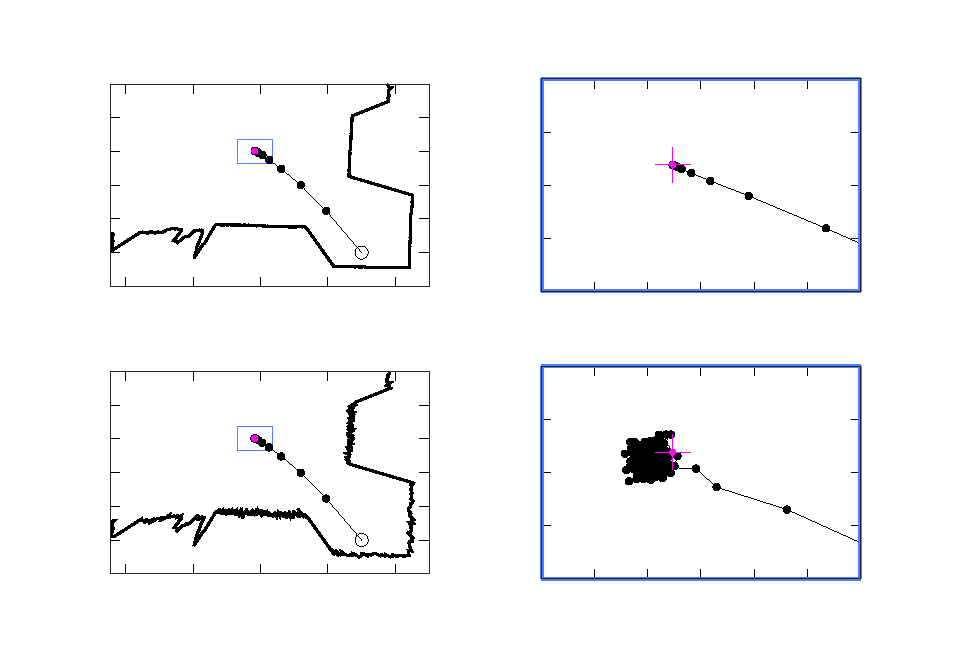
\includegraphics{./figures/parts/02/chapters/04/sections/03/translation_map_convergence}}%
    \gplfronttext
  \end{picture}%
\endgroup

\caption{\small Οι τροχιές της εκτίμησης θέσης βάσει εφαρμογής του θεωρήματος
         \ref{prop:theorem_without_disturbance} για επίπεδο διαταραχών
         αποστάσεων $\sigma_R = \sigma_V = 0.0$ m (άνω σειρά) και
         $\sigma_R = \sigma_V = 0.05$ m (κάτω σειρά). Τα τελικά σφάλματα
         εκτίμησης θέσης είναι $2.04$e-$07$ m και $5.72$e-$03$ m αντίστοιχα.
         Η εκτίμηση θέσης συγκλίνει ομοιόμορφα ασυμπτωτικά στην πρώτη περίπτωση,
         ενώ στη δεύτερη είναι ομοιόμορφα φραγμένη σε μία γειτονιά της
         πραγματικής θέσης (θεώρημα \ref{prop:theorem_with_disturbance})}
\label{fig:02_04_03:map_convergence}
\end{figure}

Ο αλγόριθμος \ref{alg:icte} παραθέτει σε ψευδοκώδικα τη μέθοδο εκτίμησης της
θέσης για δεδομένη και γνωστή εκτίμηση προσανατολισμού.

\begin{algorithm}[h]
  \caption{\texttt{icte}}
  \begin{spacing}{1.3}
    \begin{algorithmic}[1]
      \REQUIRE $\bm{M}$, $\mathcal{S}_R$, $\hat{\bm{p}}(\hat{x}, \hat{y}, \hat{\theta})$, $k_{max}$, $\varepsilon_u$, $N_s$
      \ENSURE $\hat{\bm{p}}^\prime(\hat{x}^{\prime}, \hat{y}^{\prime}, \hat{\theta})$
      \STATE $k \leftarrow 0$
      \WHILE {$k < k_{max}$}
      \STATE $\mathcal{S}_V^{[k]} \leftarrow \texttt{scan\_map}(M, \hat{\bm{p}}, N_s)$
      \STATE $X_1 \leftarrow \texttt{diff\_dft}(\mathcal{S}_R, \mathcal{S}_V^{[k]})$
      \STATE $(X_{1,r}, X_{1,i}) \leftarrow (\texttt{re}(X_1), \texttt{im}(X_1))$
      \STATE $\bm{u}_k = \begin{bmatrix}
              u_x \\ u_y
             \end{bmatrix}
             =
             \dfrac{1}{N_s}
             \begin{bmatrix}
               \cos\hat{\theta} & \sin\hat{\theta} \\
               \sin\hat{\theta} & -\cos\hat{\theta}
             \end{bmatrix}
             \begin{bmatrix}
               X_{1,r} \\ X_{1,i}
             \end{bmatrix}
             $
      \STATE $\hat{\bm{p}}\leftarrow \hat{\bm{p}}+ \bm{u}_k$
      \IF {$\|\bm{u}_k\|_2 < \varepsilon_u$}
        \STATE \texttt{break}
      \ENDIF
      \STATE $k \leftarrow k + 1$
      \ENDWHILE
      \STATE $\hat{\bm{p}}^\prime \leftarrow \hat{\bm{p}}$
      \RETURN $\hat{\bm{p}}^\prime$
    \end{algorithmic}
  \end{spacing}
  \label{alg:icte}
\end{algorithm}

\begin{algorithm}[h]
  \caption{\texttt{diff\_dft}}
  \begin{spacing}{1.3}
    \begin{algorithmic}[1]
      \REQUIRE $\mathcal{S}_R, \mathcal{S}_V$
      \ENSURE $X_1$
      \STATE \texttt{assert} $|\mathcal{S}_R| = |\mathcal{S}_{v}^{[k]}|$
      \STATE $N_s \leftarrow |\mathcal{S}_R|$
      \STATE {$\bm{\Delta} \leftarrow \{\varnothing\}$}
      \FOR{$n = 0:N_s-1$}
      \STATE $d_n \leftarrow \mathcal{S}_R[n] - \mathcal{S}_{v}^{[k]}[n]$
      \STATE \texttt{append} $d$ to $\bm{\Delta}$
      \ENDFOR
      \STATE $\bm{X} \leftarrow \texttt{DFT}(\bm{\Delta})$
      \STATE $X_1 \leftarrow \bm{X}[1]$
      \RETURN $X_1$
    \end{algorithmic}
  \end{spacing}
  \label{alg:diff_dft}
\end{algorithm}


